%%%%%%%%%%%%%%%%%%%%%%%%%%%%%%%%%%%%%%%%%%%%%%%%%%%%%%%%%%%%%%%%%%%%%%%%%%%%%%%%
% Relatório final — GDSCO0055 Introdução ao Processamento Digital de Imagens
% Formato replicado do modelo em modelo_relatorio/ (tcc.cls + dados_tcc.tex + tcc.tex)
% num arquivo único. Compilar com:  pdflatex relatorio.tex  (duas vezes, por causa das referências)
%%%%%%%%%%%%%%%%%%%%%%%%%%%%%%%%%%%%%%%%%%%%%%%%%%%%%%%%%%%%%%%%%%%%%%%%%%%%%%%%

\documentclass[12pt]{article}

% ── conteúdo de tcc.cls ──────────────────────────────────────────────────────
\usepackage[utf8]{inputenc}
\usepackage[T1]{fontenc}
\usepackage[portuguese,brazil]{babel}
\usepackage{titlesec}
\usepackage{titling}
\usepackage{graphicx}
\usepackage{indentfirst}
\usepackage{float}
\usepackage{setspace}
\usepackage{afterpage}
\usepackage{tabularx}
\usepackage{fancyhdr}
\usepackage[labelfont=bf,textfont=bf]{caption}
\usepackage[a4paper, left = 1.18in, right = 0.79in, top = 1.18in, bottom = 0.79in]{geometry}

\newcommand\blankpage{%
    \null
    \thispagestyle{empty}%
    \addtocounter{page}{-1}%
    \newpage}

\parindent=0.49in
\parskip=6pt
\onehalfspacing

\makeatletter
\renewcommand\section{\@startsection{section}{1}{\z@}%
                       {-18\p@ \@plus -4\p@ \@minus -4\p@}%
                       {12\p@ \@plus 4\p@ \@minus 4\p@}%
                       {\newpage\normalfont\large\bfseries\boldmath
                        \rightskip=\z@ \@plus 8em\pretolerance=10000 }}
\renewcommand\subsection{\@startsection{subsection}{2}{\z@}%
                       {-18\p@ \@plus -4\p@ \@minus -4\p@}%
                       {8\p@ \@plus 4\p@ \@minus 4\p@}%
                       {\normalfont\normalsize\bfseries\boldmath
                        \rightskip=\z@ \@plus 8em\pretolerance=10000 }}
\renewcommand\paragraph{\@startsection{paragraph}{4}{\z@}%
                       {-12\p@ \@plus -4\p@ \@minus -4\p@}%
                       {-0.5em \@plus -0.22em \@minus -0.1em}%
                       {\normalfont\normalsize\itshape}}
\makeatother

% ── pacotes de tcc.tex ───────────────────────────────────────────────────────
\usepackage{hyperref}
\usepackage{amsmath}
\usepackage{listings}
\usepackage{booktabs}
\usepackage{multirow}
\usepackage{xcolor}

\graphicspath{{figuras/}}
\newcommand{\pendente}[1]{\textcolor{red}{\textbf{[PENDENTE: #1]}}}

% ── conteúdo de dados_tcc.tex ────────────────────────────────────────────────
\author{Guilherme Nogueira da Silva}
\title{Mapas de Calor de Jogadores de Futebol a partir de Vídeo}
\newcommand{\subtitulo}{Segmentação por cor, classificação de times por histograma e mapeamento por homografia}
\newcommand{\nomedocurso}{Introdução ao Processamento Digital de Imagens}
\newcommand{\professor}{Leonardo Vidal Batista}

\begin{document}
\pagestyle{empty}

% ════════════════════════════════════════════════════════════════════════════
% CAPA
% ════════════════════════════════════════════════════════════════════════════
\begin{center}
\LARGE{\bf Mapas de Calor de Jogadores de Futebol a partir de Vídeo}\\[0.5em]
\large{\subtitulo}\\[1em]
\Large{\bf \nomedocurso}\\
\large{GDSCO0055 --- Prof.\ \professor}
\end{center}

\vspace{1em}

\begin{center}
Guilherme Nogueira da Silva
\end{center}

\vfill

\begin{figure}[H]
\centering

\includegraphics{logo2.jpg}
\end{figure}

\begin{center}
CENTRO DE INFORMÁTICA \\
UNIVERSIDADE FEDERAL DA PARAÍBA
\end{center}

\vspace{2in}

\begin{center}
João Pessoa, \the\year
\end{center}

\newpage
\pagestyle{plain}

% ════════════════════════════════════════════════════════════════════════════
\section{INTRODUÇÃO}
% ════════════════════════════════════════════════════════════════════════════

O mapa de calor (\textit{heatmap}) de um jogador de futebol mostra em quais regiões
do campo ele passou mais tempo ao longo de uma partida. É uma das visualizações mais
usadas em análise tática, mas normalmente depende de sistemas de rastreamento
dedicados (câmeras calibradas, GPS) ou de anotação manual. Este trabalho constrói esse
mapa a partir de um vídeo comum de transmissão, usando técnicas de Processamento
Digital de Imagens.

O problema envolve três perguntas para cada instante do vídeo: \emph{onde estão os
jogadores na imagem}, \emph{a qual time cada um pertence} e \emph{a que ponto do
campo real corresponde cada posição da imagem}. A primeira é resolvida por uma rede
neural pré-treinada (YOLO), usada somente para detectar pessoas. Todas as demais
etapas --- segmentação do gramado, separação dos times pela cor do uniforme,
mapeamento geométrico da imagem para o campo e construção do mapa --- são feitas com
técnicas clássicas da disciplina \cite{gonzalez2018}, implementadas de forma explícita e com os
parâmetros justificados por medições.

Como fonte de dados usamos o SoccerNet \textit{Game State Reconstruction}
\cite{somers2024}, que fornece, além do vídeo, a posição de cada jogador na imagem e
no campo, o time e o papel (jogador, goleiro, árbitro) de cada pessoa em todos os
quadros. Isso permite medir quantitativamente cada etapa do pipeline, e não apenas
avaliá-la visualmente.

Este relatório está organizado da seguinte forma: a Seção~2 descreve os dados e o
método de cada etapa; a Seção~3 apresenta os resultados medidos contra o gabarito; a
Seção~4 discute as limitações encontradas; e a Seção~5 conclui o trabalho.

% ════════════════════════════════════════════════════════════════════════════
\section{METODOLOGIA}
% ════════════════════════════════════════════════════════════════════════════

% ── 2.1 ──────────────────────────────────────────────────────────────────────
\subsection{Dados}

O SoccerNet \textit{Game State Reconstruction} (GSR) \cite{somers2024} é composto por
sequências de 30~s de partidas da primeira divisão suíça, em resolução
$1920\times1080$ a 25 quadros por segundo (750 quadros por sequência). Cada
sequência traz, por quadro, a caixa delimitadora de cada pessoa em campo, seu
identificador, papel (jogador, goleiro, árbitro), time (esquerda/direita) e a posição
dos pés em metros no plano do campo.

O desenvolvimento foi feito em uma única sequência, aqui chamada de
\texttt{clip01} (SNGS-056, conjunto de validação), escolhida por ter a câmera parada
na maior parte do tempo: é uma cobrança de falta próxima à grande área, com 15
pessoas em campo (dois times, um goleiro e um árbitro). Para verificar se os
parâmetros generalizam, três sequências de jogo corrido do mesmo conjunto
(SNGS-054, SNGS-040 e SNGS-026) foram usadas apenas como validação.

% ── 2.2 ──────────────────────────────────────────────────────────────────────
\subsection{Visão Geral do Pipeline}

O pipeline recebe o vídeo e executa as seguintes etapas:

\begin{enumerate}
  \item \textbf{Segmentação do gramado} por limiarização no espaço HSV e morfologia;
  \item \textbf{Detecção de pessoas} com YOLO, mantendo apenas as que estão sobre o gramado;
  \item \textbf{Rastreamento} com ByteTrack, que atribui um identificador persistente a cada jogador;
  \item \textbf{Classificação de times} pela cor do uniforme, com k-means e votação temporal;
  \item \textbf{Homografia} imagem$\rightarrow$campo, a partir de pontos marcados manualmente;
  \item \textbf{Mapa de calor}: projeção dos pés no campo, acumulação numa grade,
        suavização e pseudocoloração.
\end{enumerate}

Todos os parâmetros ficam num único arquivo de configuração
(\texttt{configs/default.yaml}), cada um acompanhado da medição que justifica o seu
valor. A Tabela~\ref{tab:conteudo} relaciona cada etapa com o conteúdo da
disciplina.

\begin{table}[H]
\centering
\caption{Etapas do pipeline e conteúdos da disciplina.}
\label{tab:conteudo}
\begin{tabular}{@{}ll@{}}
\toprule
\textbf{Etapa} & \textbf{Conteúdo} \\
\midrule
Conversão BGR$\rightarrow$HSV/Lab, cor do uniforme & Sistemas de cores \\
Limiarização da máscara do gramado & Operações pontuais \\
Abertura e fechamento da máscara & Morfologia matemática \\
Histograma H--S do uniforme, escolha dos limiares & Processamento de histograma \\
Homografia, escala do campo & Operações geométricas \\
Kernel gaussiano no mapa de calor & Correlação e convolução \\
Suavização do mapa no domínio da frequência & DFT, filtragem na frequência \\
Grade discreta do campo & Amostragem e quantização \\
Colormap do mapa de calor & Pseudocoloração \\
\bottomrule
\end{tabular}
\end{table}

% ── 2.3 ──────────────────────────────────────────────────────────────────────
\subsection{Segmentação do Gramado}

A máscara do gramado serve para descartar detecções fora de campo (torcida, banco,
fotógrafos) e para remover a grama dos recortes de uniforme. O quadro é convertido de
BGR para HSV, e um pixel é considerado gramado quando

\begin{equation}
H \in [h_{\min}, h_{\max}], \quad S \ge s_{\min}, \quad V \ge v_{\min},
\end{equation}

com $H$ na escala do OpenCV (0--179). Os mínimos de saturação e brilho descartam
pixels acinzentados ou escuros, cujo matiz é instável. A faixa de matiz é escolhida a
partir do histograma do canal $H$ de quadros amostrados do vídeo
(Figura~\ref{fig:hist}).

A máscara crua tem ruído: pixels verdes isolados na torcida e falhas sobre as linhas
brancas e os jogadores. Ela é limpa com uma abertura morfológica (remove ruído fora
do campo), um fechamento (une as falhas), a seleção do maior componente conexo e o
preenchimento dos buracos internos (Figura~\ref{fig:mascara}). Jogadores cortados pela borda inferior do quadro
deixavam reentrâncias abertas na máscara, que o preenchimento não alcançava; isso foi
resolvido acrescentando uma linha de gramado abaixo da imagem antes de buscar os
contornos.

% ── 2.4 ──────────────────────────────────────────────────────────────────────
\subsection{Detecção de Jogadores}

A detecção usa o YOLO11n \cite{yolo11} pré-treinado no COCO, mantendo apenas a
classe \textit{pessoa}. Nenhum ajuste fino foi feito. Cada detecção é descrita pelo
seu \textbf{ponto do pé}, o centro da base da caixa $\left(\frac{x_1+x_2}{2},
y_2\right)$, que é o ponto que toca o plano do gramado e, portanto, o único que a
homografia projeta corretamente.

Uma detecção é mantida quando tem confiança $\ge 0{,}3$, área $\ge 150$~px$^2$ e o
ponto do pé está sobre a máscara do gramado dilatada em 10~px. A dilatação tolera o
contorno serrilhado da máscara junto às placas de publicidade, onde o pé do goleiro
caía alguns pixels fora.

% ── 2.5 ──────────────────────────────────────────────────────────────────────
\subsection{Rastreamento}

O rastreamento usa o ByteTrack \cite{zhang2022bytetrack}, na implementação da
biblioteca \texttt{supervision}. Ele prevê a posição de cada jogador com um filtro de
Kalman e associa as detecções do quadro seguinte pela sobreposição (IoU) das caixas.
Os parâmetros são: confiança mínima de 0,5 para abrir um novo identificador, 3~s de
espera antes de descartar um jogador perdido e custo máximo de associação
$1 - \text{IoU} = 0{,}8$. Todos os quadros são processados (passo 1).

Para o mapa de calor por time, um identificador que se \emph{divide} em vários é
inofensivo, mas um identificador que \emph{mistura} dois jogadores de times
diferentes contamina a classificação. Por isso, além do número de trocas de
identificador, medimos a \textbf{pureza}: a fração das associações em que o
identificador previsto corresponde ao seu jogador majoritário no gabarito.

% ── 2.6 ──────────────────────────────────────────────────────────────────────
\subsection{Modelo do Campo e Homografia}

O campo é modelado com as medidas da regra (Lei 1 da IFAB): $105\times68$~m, com
origem no canto superior esquerdo, $X$ ao longo do comprimento e $Y$ ao longo da
largura. A partir das medidas oficiais (grande área de $16{,}5\times40{,}32$~m,
pequena área de $5{,}5\times18{,}32$~m, círculo central e meia-lua com raio de
9,15~m, marca do pênalti a 11~m) são definidos 35 pontos notáveis
(Figura~\ref{fig:campo}).

Como o gramado é um plano, pontos da imagem $(x, y)$ e do campo $(X, Y)$ se
relacionam por uma homografia $\mathbf{H}$ ($3\times3$), em coordenadas homogêneas:

\begin{equation}
\begin{bmatrix} X' \\ Y' \\ w \end{bmatrix} = \mathbf{H}
\begin{bmatrix} x \\ y \\ 1 \end{bmatrix}, \qquad
(X, Y) = \left(\frac{X'}{w}, \frac{Y'}{w}\right).
\end{equation}

Cada correspondência fornece duas equações lineares nos nove elementos
$\mathbf{h}$ de $\mathbf{H}$:

\begin{equation}
\begin{bmatrix}
-x & -y & -1 & 0 & 0 & 0 & Xx & Xy & X \\
0 & 0 & 0 & -x & -y & -1 & Yx & Yy & Y
\end{bmatrix} \mathbf{h} = \mathbf{0}.
\end{equation}

Com $n \ge 4$ pontos, empilham-se as equações numa matriz $\mathbf{A}$
($2n\times9$), e a solução de mínimos quadrados com $\lVert\mathbf{h}\rVert = 1$ é o
vetor singular direito associado ao menor valor singular de $\mathbf{A}$
(\textit{Direct Linear Transform}, DLT \cite{hartley2004}). Antes disso, os pontos
de cada conjunto são normalizados (centróide na origem e distância média
$\sqrt{2}$), o que melhora o condicionamento numérico \cite{hartley1997}. Essa
versão didática foi implementada com NumPy e comparada com
\texttt{cv2.findHomography}; no pipeline usa-se a versão do OpenCV com RANSAC
\cite{fischler1981}, que descarta automaticamente um clique errado (limiar de 1~m).

Os pontos são marcados manualmente com uma ferramenta própria: o usuário clica num
ponto do gramado no primeiro quadro e depois no ponto correspondente do modelo do
campo. A partir do quarto par, as linhas do modelo são projetadas de volta sobre o
quadro com $\mathbf{H}^{-1}$, e o alinhamento com as linhas reais é a principal
verificação visual. Pontos do campo que ficam atrás da câmera (coordenada $w$ com
sinal oposto ao de um ponto visível) são descartados do desenho.

Uma homografia fixa só vale enquanto a câmera está parada. No \texttt{clip01} a
câmera passa a acompanhar o lance a partir do quadro 576 (Seção~\ref{sec:res_h}).
Por isso, nesta versão, o mapa de calor usa apenas os quadros 0--575. A propagação
da homografia entre quadros, que permitiria usar o clipe inteiro, é trabalho em
andamento.

% ── 2.7 ──────────────────────────────────────────────────────────────────────
\subsection{Classificação de Times}

Para cada pessoa rastreada, recorta-se a região do tronco: de 20\% a 60\% da altura
e de 20\% a 80\% da largura da caixa, evitando cabeça, calção e a grama dos lados.
Os pixels de gramado do recorte são removidos com a mesma máscara HSV da
Seção~2.3. Comparamos quatro descritores de cor dos pixels restantes:

\begin{itemize}
  \item \textbf{RGB médio}: média dos canais B, G e R (referência ingênua);
  \item \textbf{Lab médio}: média de $L^*$, $a^*$ e $b^*$;
  \item \textbf{$a^*b^*$ médio}: apenas os canais de cromaticidade do Lab, descartando
        a luminância $L^*$;
  \item \textbf{Histograma H--S}: histograma 2D de matiz e saturação com
        $16\times8$ classes, normalizado para soma 1 (ignora o brilho $V$).
\end{itemize}

Os descritores dos 50 primeiros quadros são agrupados por k-means com $k=2$
(semente fixa); depois, cada detecção recebe o grupo do centróide mais próximo. O
número do grupo é arbitrário, e a correspondência grupo$\rightarrow$time é feita uma
única vez.

Por fim, aplica-se uma \textbf{votação temporal} por identificador. Em vez da moda
sobre o identificador inteiro, usa-se uma moda em janela deslizante: o rótulo de um
identificador no quadro $t$ é

\begin{equation}
\hat{c}_t = \operatorname{moda}\{\, c_s \;:\; |s - t| \le w \,\},
\end{equation}

considerando apenas os quadros $s$ do mesmo identificador, com $w$ = 1~s
(25~quadros). Esse filtro de moda 1D corrige erros isolados sem propagar o rótulo
através de uma troca de identificador (Seção~\ref{sec:res_times}).

% ── 2.8 ──────────────────────────────────────────────────────────────────────
\subsection{Mapa de Calor}

\pendente{etapa em implementação.} O plano é: projetar o ponto do pé de cada jogador
com $\mathbf{H}$ em cada quadro válido; acumular as posições numa grade de
$0{,}5$~m ($210\times136$ células), normalizando pelo número de quadros (tempo de
permanência); suavizar o mapa com um kernel gaussiano, tanto por convolução
espacial (implementada manualmente e comparada com \texttt{cv2.GaussianBlur}) quanto
no domínio da frequência (DFT, filtro passa-baixa gaussiano, DFT inversa),
verificando a equivalência prevista pelo teorema da convolução; e aplicar um
colormap sobre o desenho do campo.

% ── 2.9 ──────────────────────────────────────────────────────────────────────
\subsection{Protocolo de Avaliação e Ferramentas}

Em cada quadro, as caixas previstas são associadas às do gabarito pelo algoritmo
húngaro sobre a IoU, aceitando pares com IoU $\ge 0{,}5$. A partir dessa associação
medem-se: recall e precisão da detecção; trocas de identificador e pureza do
rastreamento; e acurácia da classificação de times sobre os jogadores de linha. O
erro da homografia é medido em metros, projetando os pés do gabarito com
$\mathbf{H}$ e comparando com a posição real no campo.

\begin{itemize}
  \item \textbf{Python 3}, \textbf{OpenCV} e \textbf{NumPy}: núcleo do processamento de imagens;
  \item \textbf{Ultralytics} (YOLO11n) e \textbf{supervision} (ByteTrack);
  \item \textbf{scikit-learn} (k-means) e \textbf{SciPy} (algoritmo húngaro);
  \item \textbf{matplotlib}: figuras;
  \item \textbf{pytest}: testes das funções determinísticas (homografia com pontos
        sintéticos, máscara, votação etc.).
\end{itemize}

Os tempos foram medidos em CPU (Intel Core i7-1355U), sem GPU.

% ════════════════════════════════════════════════════════════════════════════
\section{RESULTADOS}
% ════════════════════════════════════════════════════════════════════════════

% ── 3.1 ──────────────────────────────────────────────────────────────────────
\subsection{Segmentação do Gramado}

O histograma do canal $H$ (Figura~\ref{fig:hist}) mostra a grama concentrada entre
$H \approx 35$ (grama ao sol, tendendo ao amarelo) e $H \approx 66$ (grama na sombra).
O pico em $H = 30$--$32$ vem da torcida e das faixas amarelas do estádio. Inicialmente
usamos $h_{\min} = 35$, mas esse valor fica exatamente sobre o pico da grama ao sol:
diferenças de um ou dois níveis entre decodificadores de vídeo bastavam para apagar
a área ensolarada da máscara. Em vez de inspecionar só um quadro, medimos a fração
de pés de jogadores do gabarito que caem dentro da máscara: com $h_{\min} = 35$ ela
era de 0,88; com $h_{\min} = 33$ passa a 0,98 nas sequências de ajuste (056 e 040) e
a 0,977 nas de validação (054 e 026). Valores abaixo de 33 não melhoram e se
aproximam do amarelo da torcida.

O limiar de brilho foi escolhido pelo 1º percentil de $V$ da grama na sombra
($V = 26$): com $v_{\min} = 40$, um terço da área sombreada desaparecia. O elemento
estruturante da morfologia tem $11\times11$~px; com $7\times7$, as linhas brancas e
os jogadores separavam pedaços do campo do componente principal. Como comparação,
o limiar automático de Otsu sobre o índice de excesso de verde
($G - \frac{R+B}{2}$) manteve apenas 0,62 dos pés dentro da máscara.

\begin{figure}[H]
    \centering
    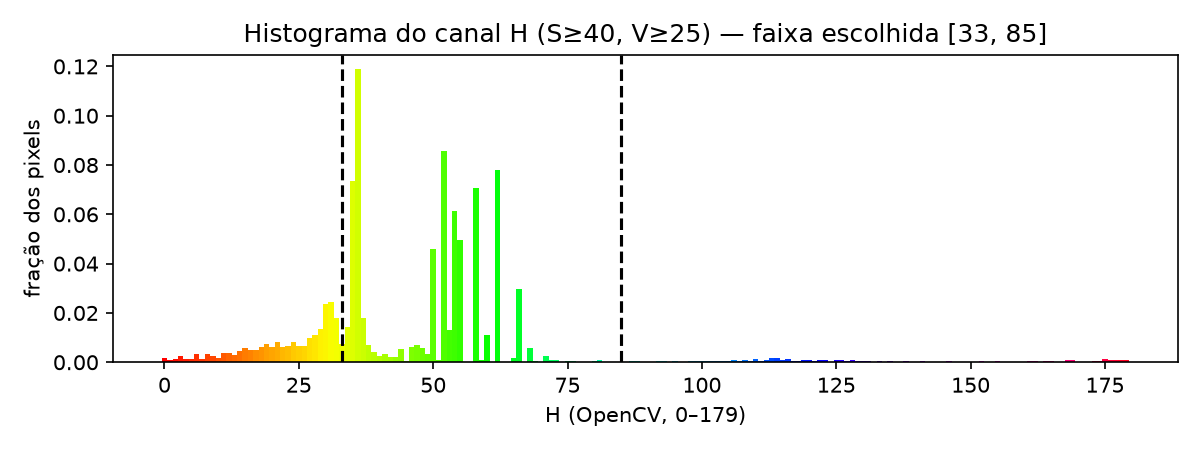
\includegraphics[width=1\linewidth]{01_histograma_h.png}
    \caption{Histograma do canal $H$ dos pixels com $S \ge 40$ e $V \ge 25$ em 10
             quadros do \texttt{clip01}. As linhas tracejadas marcam a faixa escolhida.}
    \label{fig:hist}
\end{figure}

\begin{figure}[H]
    \centering
    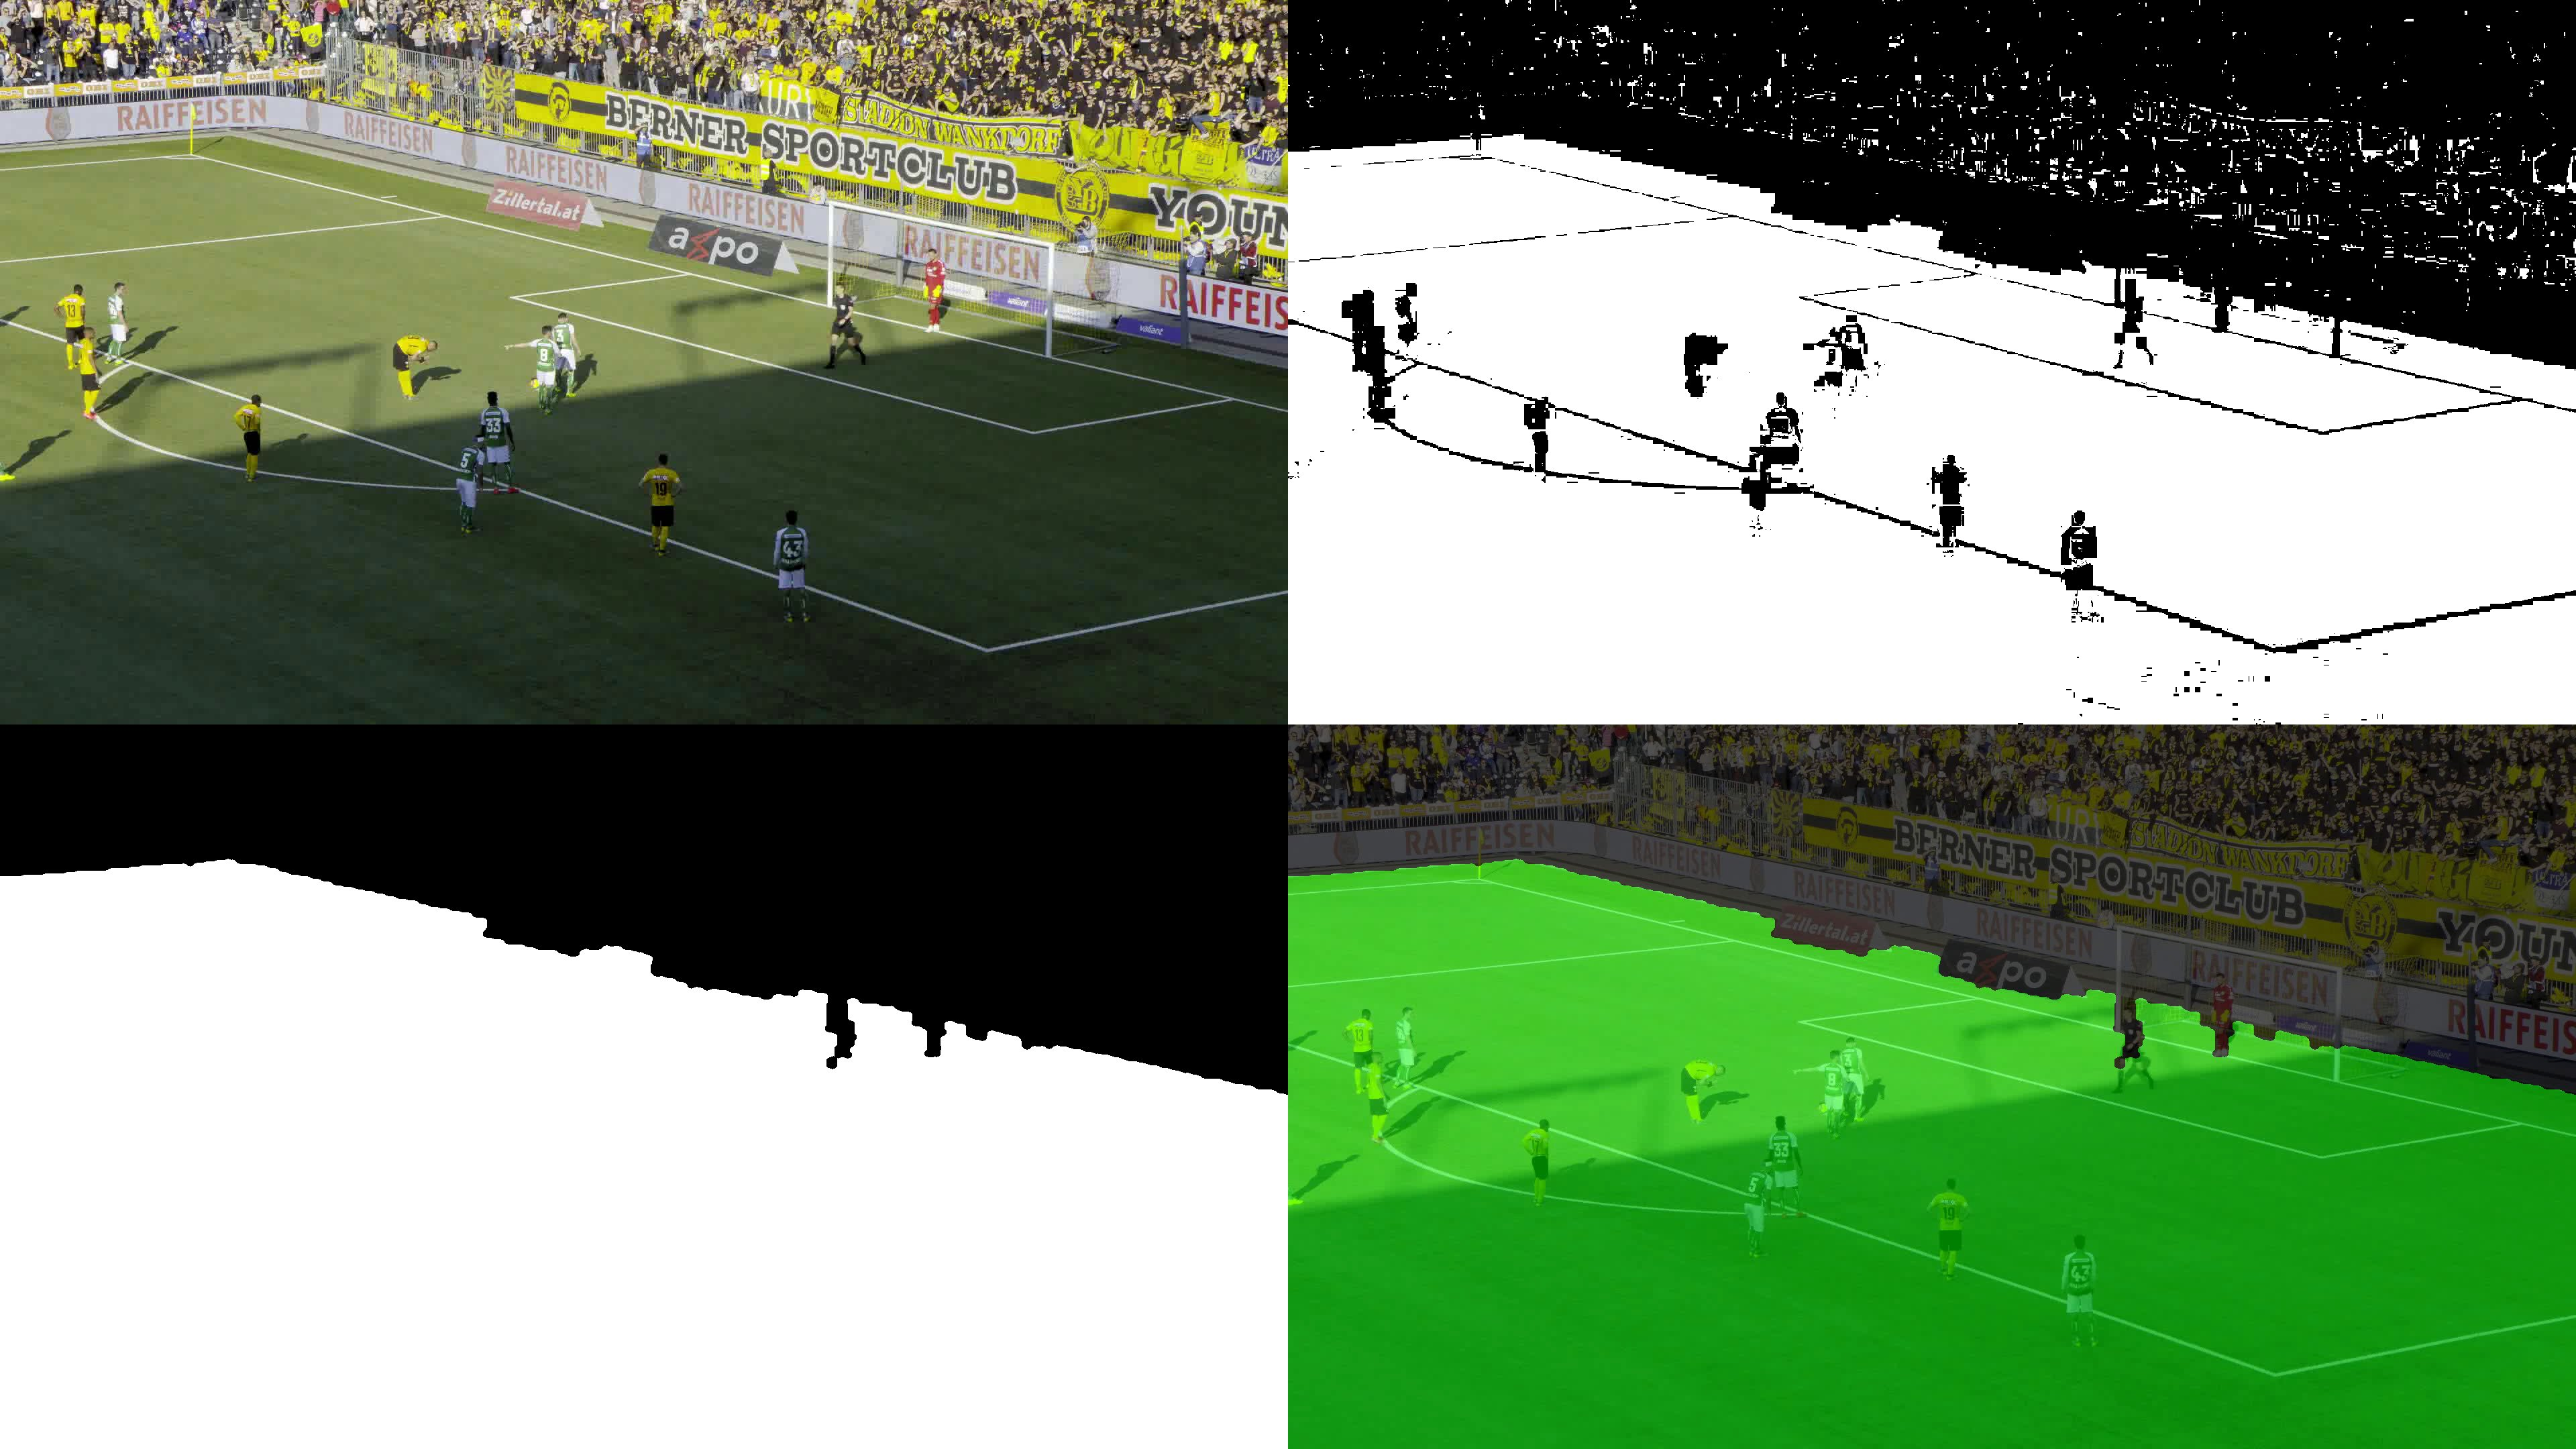
\includegraphics[width=1\linewidth]{01_mascara_gramado.jpg}
    \caption{Segmentação do gramado: quadro original; limiarização HSV crua; após
             morfologia, maior componente e preenchimento; máscara sobreposta.}
    \label{fig:mascara}
\end{figure}

% ── 3.2 ──────────────────────────────────────────────────────────────────────
\subsection{Detecção}

A Tabela~\ref{tab:imgsz} mostra o efeito da resolução de entrada do YOLO em 50
quadros do \texttt{clip01}. Jogadores distantes ocupam poucos pixels e só são
encontrados em resoluções maiores. O filtro pelo gramado praticamente não perde
jogadores e eleva a precisão de 0,875 para 0,952 em 1280~px, removendo fotógrafos,
gandulas e pessoas da torcida (Figura~\ref{fig:deteccao}). Em todos os 750 quadros
do \texttt{clip01}, a detecção filtrada tem recall de 0,933 e precisão de 0,948.

\begin{table}[H]
\centering
\caption{Resolução de entrada do YOLO11n (50 quadros do \texttt{clip01}, IoU $\ge 0{,}5$, CPU).}
\label{tab:imgsz}
\begin{tabular}{@{}rrrrr@{}}
\toprule
\textbf{Resolução} & \textbf{Recall} & \multicolumn{2}{c}{\textbf{Precisão}} & \textbf{ms/quadro} \\
 & & \textbf{sem filtro} & \textbf{com filtro} & \\
\midrule
640  & 0,817 & 0,930 & 0,931 & 49 \\
960  & 0,925 & 0,928 & 0,932 & 53 \\
1280 & \textbf{0,942} & 0,875 & \textbf{0,952} & 129 \\
\bottomrule
\end{tabular}
\end{table}

Nas três sequências de jogo corrido, o filtro custa entre 0,3 e 3,0 pontos
percentuais de recall (SNGS-026: 0,3; SNGS-040: 1,8; SNGS-054: 3,0). A principal
limitação está no próprio detector: na SNGS-040, com a câmera mais aberta, o YOLO
encontra apenas 74\% dos jogadores. Também medimos a detecção da bola, com a classe
\textit{sports ball} do COCO: o recall foi de apenas 0,51 em jogo corrido, e por
isso a bola ficou fora do escopo.

\begin{figure}[H]
    \centering
    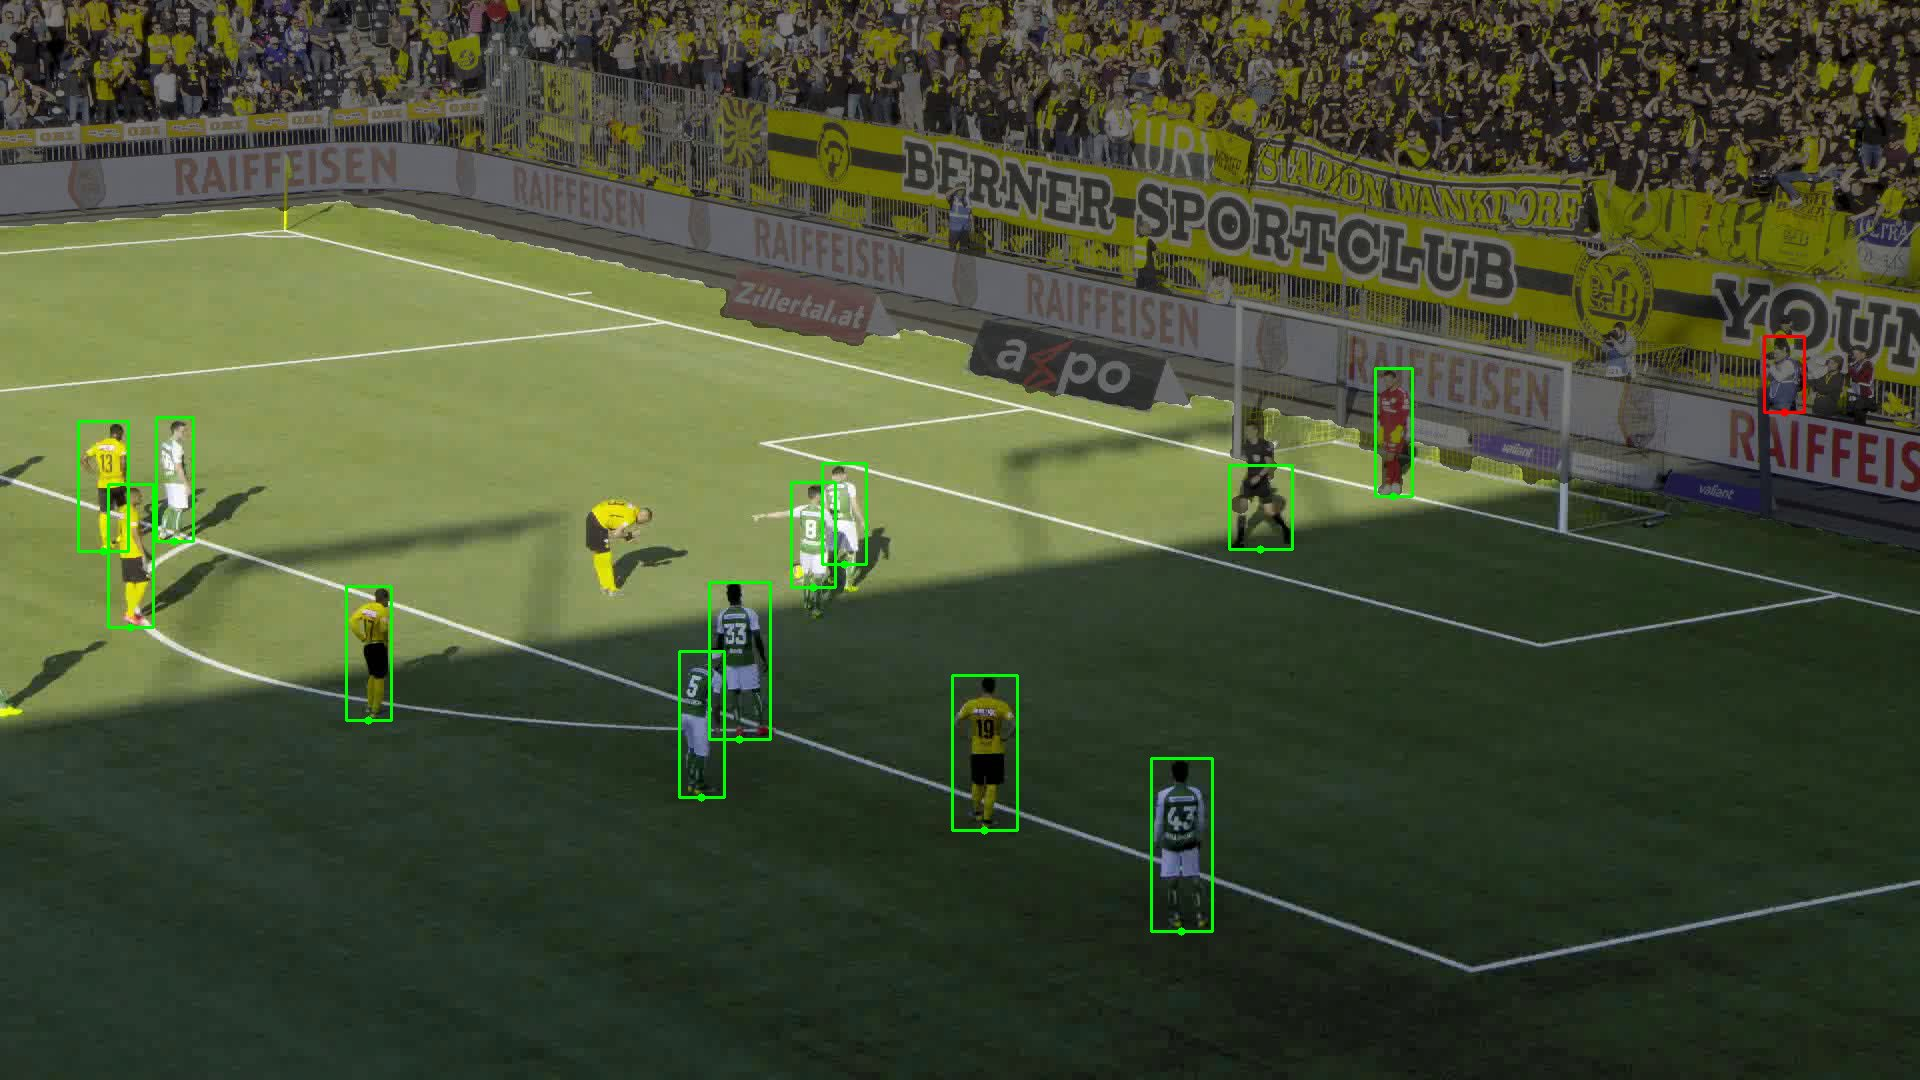
\includegraphics[width=1\linewidth]{02_deteccao.jpg}
    \caption{Detecções mantidas (verde) e descartadas pelo filtro do gramado
             (vermelho, um fotógrafo atrás da placa), com o ponto do pé de cada uma.
             O jogador curvado no centro não é detectado pelo YOLO.}
    \label{fig:deteccao}
\end{figure}

% ── 3.3 ──────────────────────────────────────────────────────────────────────
\subsection{Rastreamento}

No \texttt{clip01} (Figura~\ref{fig:tracking}), o rastreador criou 31 identificadores para as 15 pessoas do
gabarito, com 34 trocas de identificador e pureza de 0,948. A duração mediana de um
identificador é de 215 quadros (8,6~s); sete identificadores duram menos de 1~s.
Nas sequências de jogo corrido foram de 2,3 a 3,7 identificadores por jogador, com
pureza entre 0,94 e 0,97; processar todos os quadros, em vez de um a cada dois,
reduziu o número de identificadores por jogador em 20 a 30\%.

\begin{figure}[H]
    \centering
    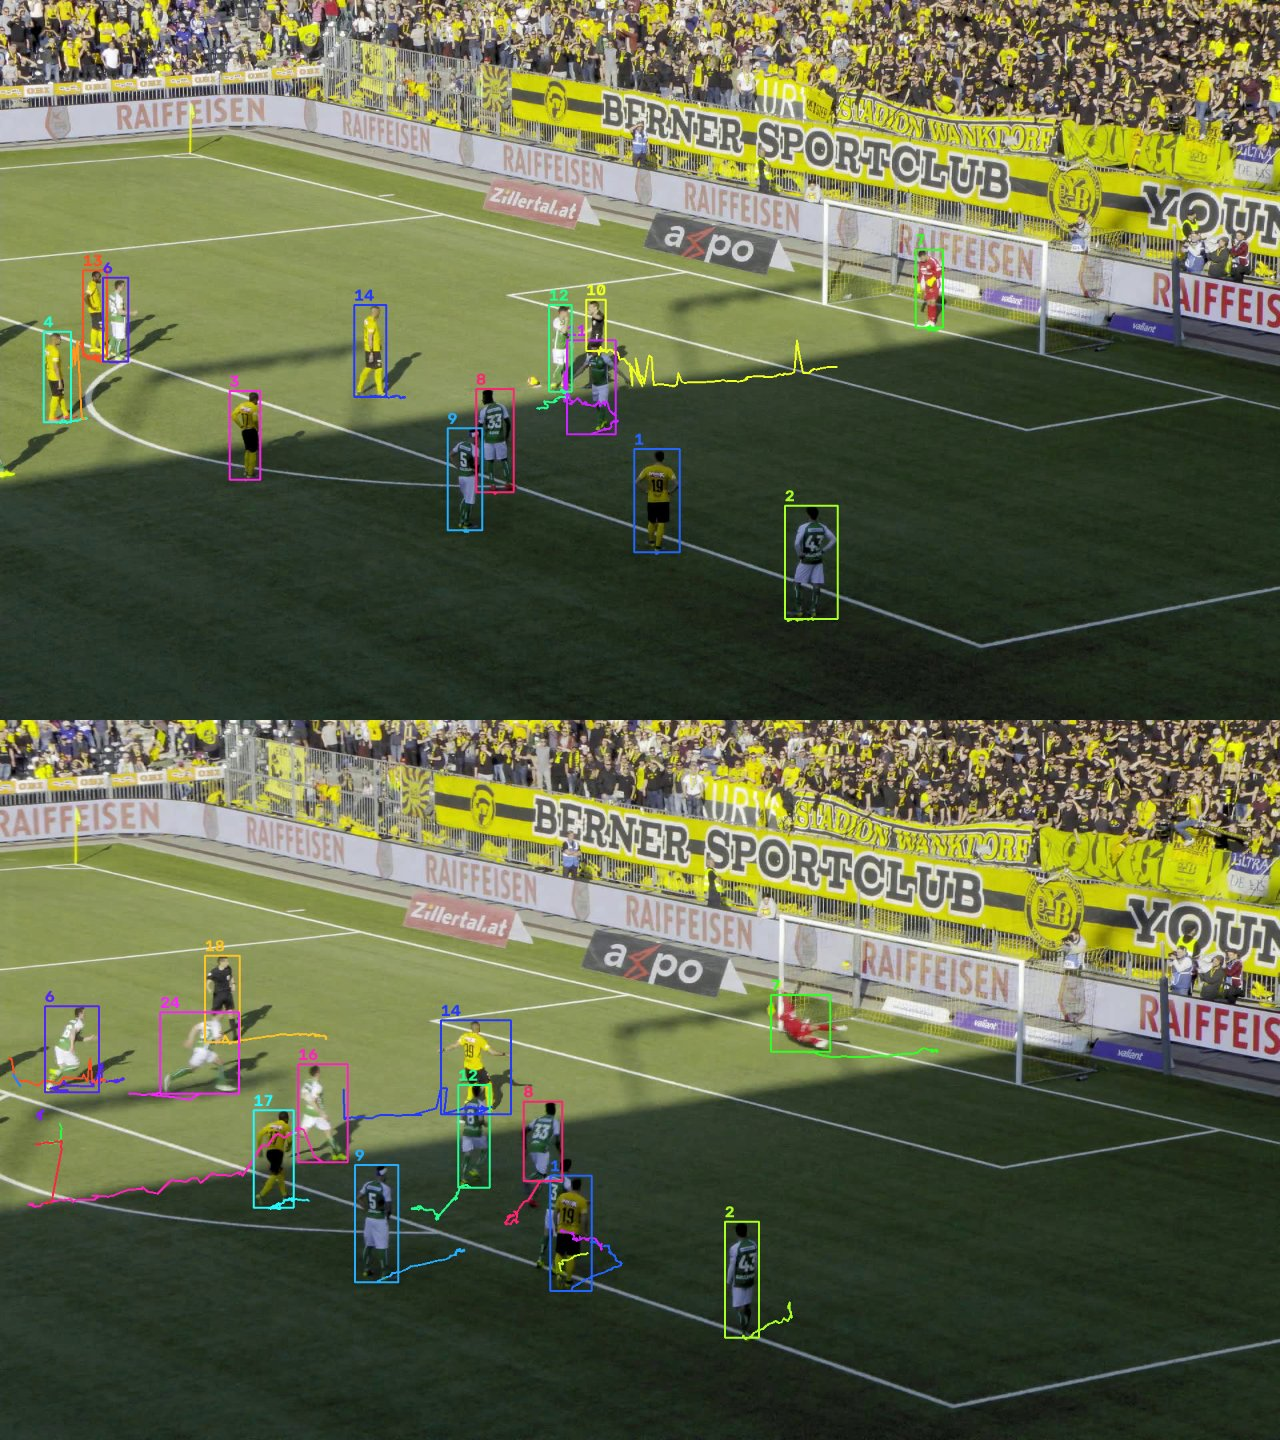
\includegraphics[width=0.85\linewidth]{03_tracking.jpg}
    \caption{Rastreamento em dois instantes do \texttt{clip01}: cada cor é um
             identificador, com o rastro recente do ponto do pé.}
    \label{fig:tracking}
\end{figure}

% ── 3.4 ──────────────────────────────────────────────────────────────────────
\subsection{Homografia}
\label{sec:res_h}

Foram marcados 11 pontos no quadro 0 do \texttt{clip01} (cantos da grande e da
pequena área, base das traves, extremidades da meia-lua e o canto do campo). O maior
erro de reprojeção entre os pontos marcados foi de 0,21~m, e nenhum foi descartado
pelo RANSAC. As linhas do modelo projetadas com $\mathbf{H}^{-1}$ coincidem com as
linhas do gramado (Figura~\ref{fig:overlay}).

Projetando os pés dos jogadores do gabarito, o erro mediano no quadro 0 é de 0,58~m.
O erro não é aleatório: quase todos os pés aparecem de 0,4 a 0,7~m mais perto da
câmera do que no gabarito, ou seja, é um deslocamento sistemático entre a nossa
marcação e a calibração do SoccerNet. Como referência, uma homografia calculada
com os próprios pés do gabarito tem erro de 0,03~m. Mesmo assim, o desvio é da
ordem de uma célula do mapa de calor (0,5~m).

Mantendo $\mathbf{H}$ fixa ao longo do clipe (Figura~\ref{fig:erro_h}), o erro fica
estável até o quadro 575 e cresce a partir do quadro 576, quando a câmera passa a
acompanhar o lance, chegando a 13,8~m no quadro 744.

\begin{figure}[H]
    \centering
    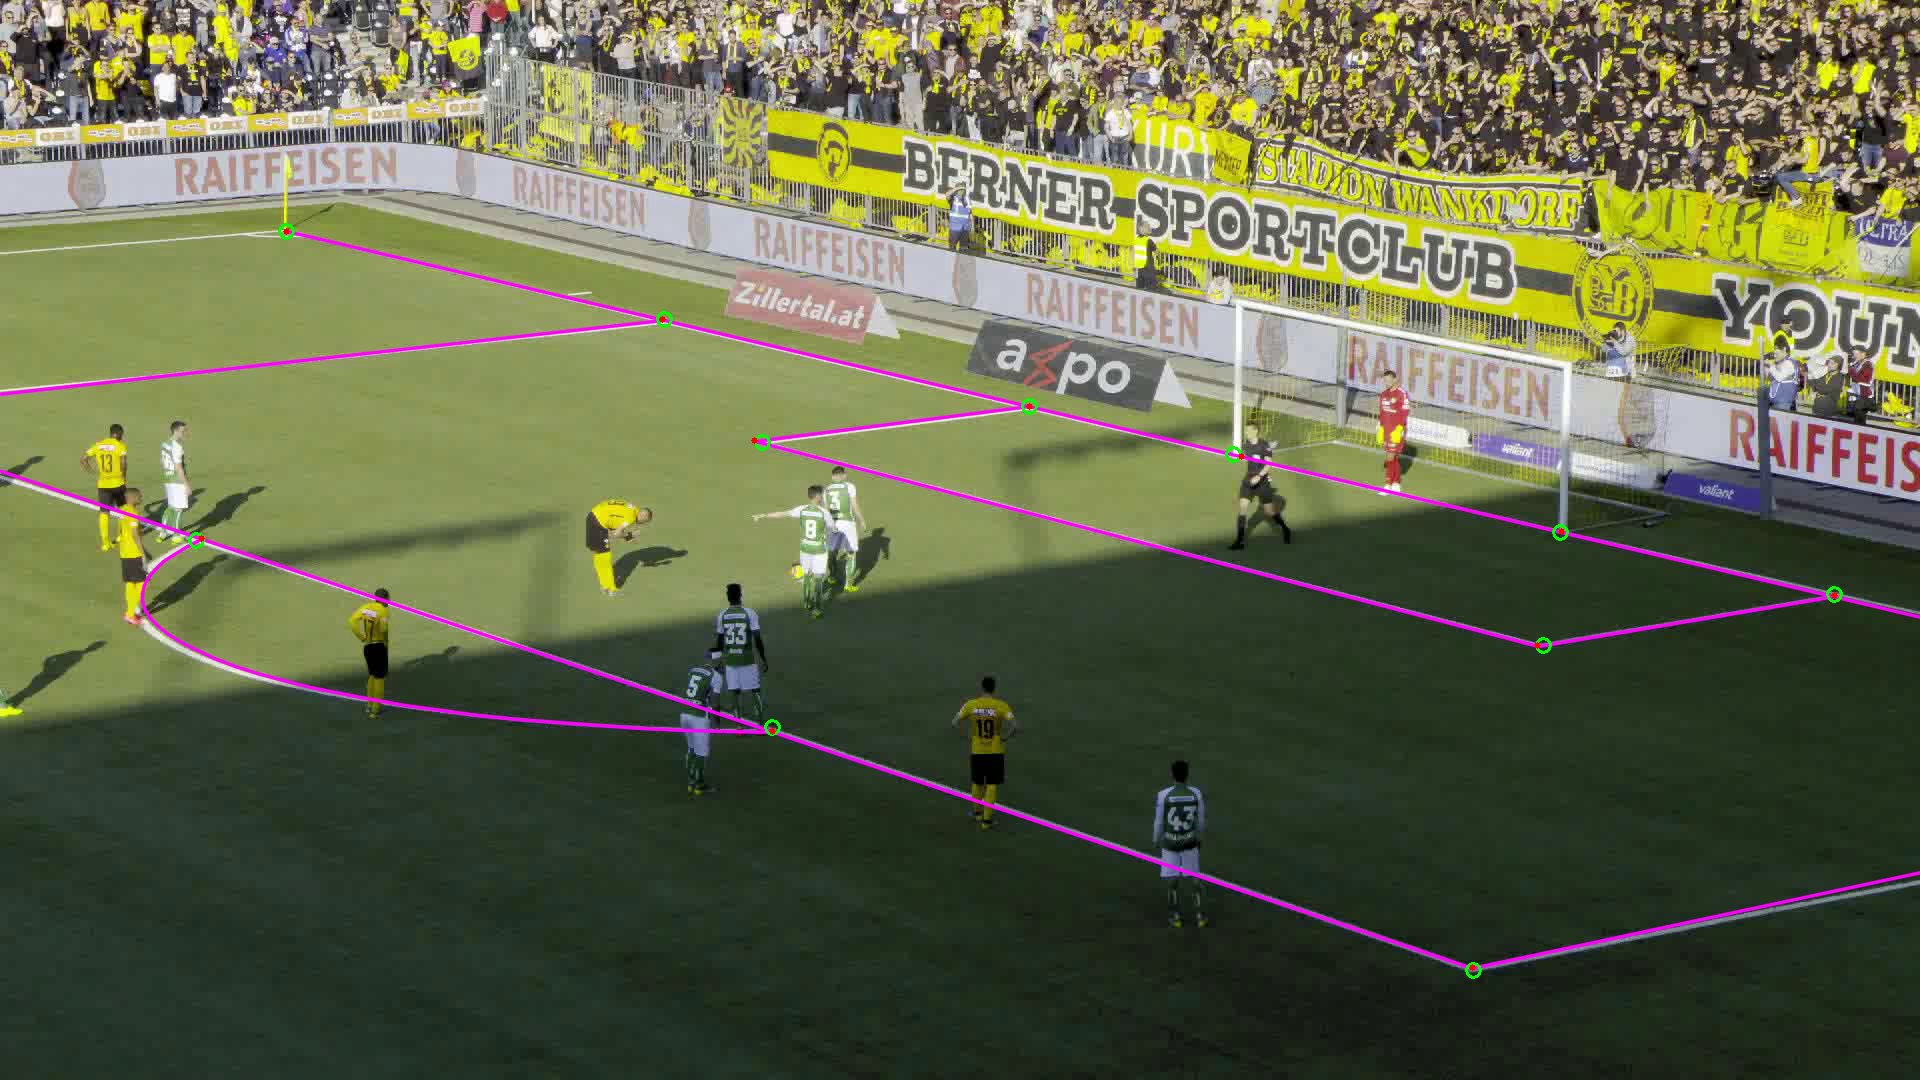
\includegraphics[width=1\linewidth]{05_homografia_clip01.jpg}
    \caption{Validação da homografia manual: linhas do modelo do campo projetadas
             sobre o quadro 0 com $\mathbf{H}^{-1}$ (magenta), pontos marcados (verde)
             e posição reprojetada dos pontos do modelo (vermelho).}
    \label{fig:overlay}
\end{figure}

\begin{figure}[H]
    \centering
    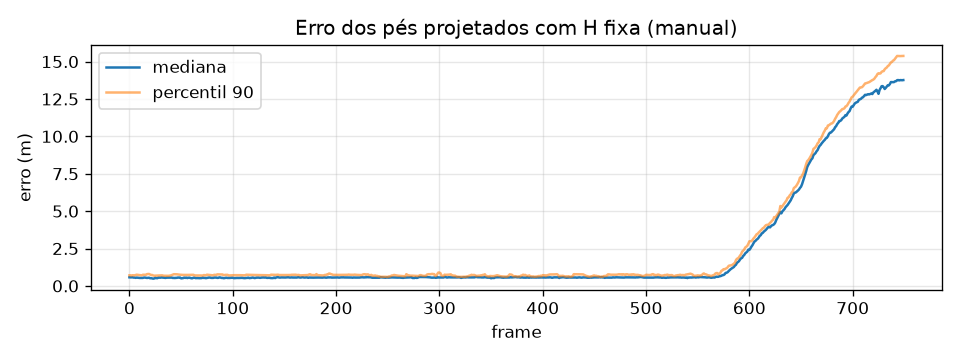
\includegraphics[width=1\linewidth]{05_erro_homografia_clip01.png}
    \caption{Erro dos pés do gabarito projetados com a homografia fixa do quadro 0,
             ao longo do \texttt{clip01}. O salto a partir do quadro 576 é o
             movimento da câmera.}
    \label{fig:erro_h}
\end{figure}

\begin{figure}[H]
    \centering
    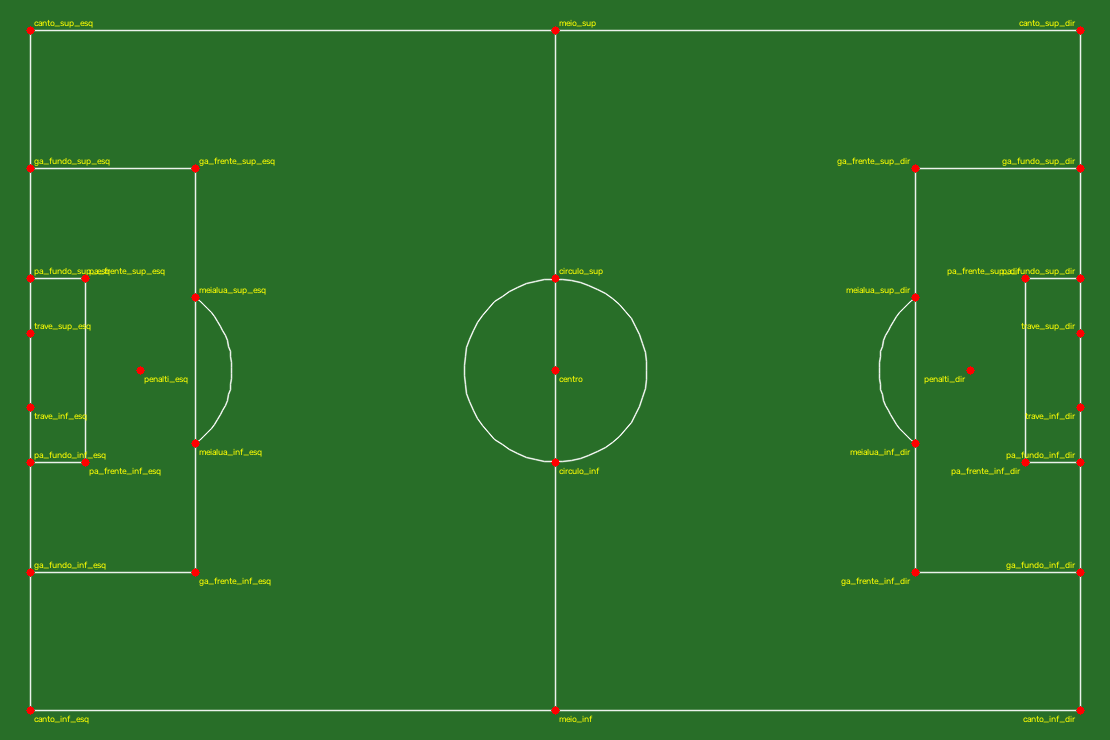
\includegraphics[width=1\linewidth]{04_campo_modelo.png}
    \caption{Modelo do campo ($105\times68$~m) com os 35 pontos notáveis usados na marcação.}
    \label{fig:campo}
\end{figure}

% ── 3.5 ──────────────────────────────────────────────────────────────────────
\subsection{Classificação de Times}
\label{sec:res_times}

A Tabela~\ref{tab:times} mostra a acurácia sobre 7.852 detecções de jogadores de
linha do \texttt{clip01} associadas ao gabarito, para cada descritor, com e sem
remoção da grama e com as duas formas de votação.

\begin{table}[H]
\centering
\caption{Acurácia da classificação de times (jogadores de linha, \texttt{clip01}, $k=2$).}
\label{tab:times}
\begin{tabular}{@{}llrrr@{}}
\toprule
\textbf{Descritor} & \textbf{Grama} & \textbf{Por quadro} & \textbf{Janela de 1~s} & \textbf{ID inteiro} \\
\midrule
\multirow{2}{*}{RGB médio}       & mantida  & 0,586 & 0,587 & 0,649 \\
                                 & removida & 0,601 & 0,604 & 0,529 \\
\multirow{2}{*}{Lab médio}       & mantida  & 0,589 & 0,589 & 0,649 \\
                                 & removida & 0,585 & 0,586 & 0,649 \\
\multirow{2}{*}{$a^*b^*$ médio}  & mantida  & 0,870 & 0,862 & 0,846 \\
                                 & removida & 0,989 & 0,994 & 0,948 \\
\multirow{2}{*}{Histograma H--S} & mantida  & 0,992 & 0,998 & 0,961 \\
                                 & removida & \textbf{0,994} & \textbf{0,999} & 0,961 \\
\bottomrule
\end{tabular}
\end{table}

Os descritores que incluem o brilho (RGB e Lab completo) acertam pouco mais do que
o acaso. A causa é visível no próprio vídeo: metade do campo está ao sol e metade
na sombra, e a luminância $L^*$ de um mesmo uniforme varia cerca de $\pm50$ entre as
duas regiões, mais do que a diferença de cor entre os times. O k-means, então,
separa \emph{sol de sombra}, e não os times (os centróides de $L^*$ ficaram em 87 e
187). Descartando a luminância, com $a^*b^*$ ou H--S, a acurácia passa de 0,98.

Remover a grama é decisivo para o descritor de média: sem a remoção, a média do
recorte é puxada para o verde e a acurácia de $a^*b^*$ cai de 0,989 para 0,870. Para
o histograma H--S o efeito é pequeno, porque os pixels de grama ocupam classes
próprias do histograma em vez de deslocar a média.

A votação pelo identificador inteiro \emph{piorou} todos os descritores bons (de
0,994 para 0,961 no H--S). Dois identificadores do rastreador trocam de jogador entre
times num cruzamento; num deles, o classificador por quadro acerta exatamente a
divisão do gabarito (542 quadros de um time e 138 do outro), mas a moda sobre o
identificador inteiro atribui os 680 quadros ao time majoritário. A janela de 1~s
corrige erros isolados sem atravessar essas trocas e leva a acurácia a 0,999. As
Figuras~\ref{fig:times} e~\ref{fig:times_ab} mostram exemplos de recortes e a distribuição de cor por grupo.

\begin{figure}[H]
    \centering
    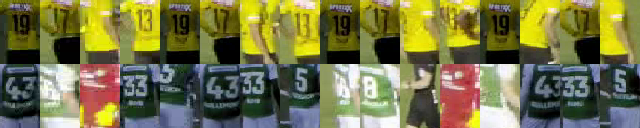
\includegraphics[width=1\linewidth]{06_times_recortes.png}
    \caption{Recortes do tronco de cada grupo após a votação. O segundo grupo reúne o
             time verde e branco, o goleiro (vermelho) e o árbitro (preto).}
    \label{fig:times}
\end{figure}

\begin{figure}[H]
    \centering
    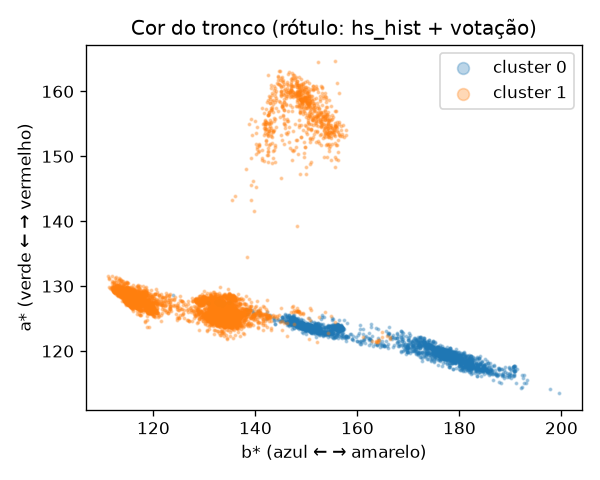
\includegraphics[width=0.7\linewidth]{06_times_ab.png}
    \caption{Cor média do tronco no plano $a^*b^*$, colorida pelo grupo atribuído
             (histograma H--S com votação). O aglomerado superior é o goleiro.}
    \label{fig:times_ab}
\end{figure}

% ── 3.6 ──────────────────────────────────────────────────────────────────────
\subsection{Mapas de Calor}

\pendente{mapas por time e por jogador; espacial vs.\ frequência (equivalência e
tempo); efeito da resolução da grade (0,25 / 0,5 / 1 / 2~m); ponto do pé vs.\ centro
da caixa.}

% ── 3.7 ──────────────────────────────────────────────────────────────────────
\subsection{Desempenho}

A Tabela~\ref{tab:tempo} mostra o tempo por quadro de cada etapa em CPU. A detecção
domina o custo (83\%); as etapas clássicas somam cerca de 26~ms por quadro.

\begin{table}[H]
\centering
\caption{Tempo médio por quadro em CPU (Intel Core i7-1355U, vídeo $1920\times1080$).}
\label{tab:tempo}
\begin{tabular}{@{}lr@{}}
\toprule
\textbf{Etapa} & \textbf{ms/quadro} \\
\midrule
Detecção (YOLO11n, 1280~px) & 121 \\
Máscara do gramado & 15 \\
Filtro das detecções & 8 \\
Decodificação e rastreamento & 3 \\
\midrule
\textbf{Total} & \textbf{$\approx$146} ($\approx$6,8 quadros/s) \\
\bottomrule
\end{tabular}
\end{table}

\pendente{tempo da classificação de times e do mapa de calor.}

% ════════════════════════════════════════════════════════════════════════════
\section{DISCUSSÃO}
% ════════════════════════════════════════════════════════════════════════════

\subsection{Iluminação e Escolha do Espaço de Cor}

O resultado mais claro deste trabalho até aqui é o efeito do espaço de cor na
separação dos times. A recomendação habitual de usar Lab por ser ``mais robusto à
iluminação'' só se confirma quando a luminância é efetivamente descartada: o Lab
completo erra tanto quanto o RGB, porque a separação entre sol e sombra no mesmo
quadro é maior do que a diferença entre os uniformes. O mesmo fenômeno apareceu na
máscara do gramado, cujo limiar inferior de matiz precisou acomodar a grama
ensolarada, mais amarelada.

\subsection{Votação Temporal e Qualidade do Rastreamento}

A votação temporal pressupõe que cada identificador corresponde a um único jogador.
Quando o rastreador mistura jogadores de times diferentes, a votação sobre o
identificador inteiro propaga o erro em vez de corrigi-lo. A janela deslizante é uma
solução simples para isso, mas o resultado mostra também que a pureza do rastreador
importa mais do que o número de identificadores: fragmentar um jogador em vários
identificadores não prejudica o mapa por time, enquanto misturar dois jogadores
prejudica.

\subsection{Árbitro e Goleiro}

Com $k=2$, o goleiro (uniforme vermelho) cai no grupo do seu próprio time, o que é
correto para o mapa por time. O árbitro, de preto, também cai nesse grupo com
qualquer um dos descritores. Aumentar $k$ para 3 ou 4 não o isolou: o k-means
preferiu dividir um time entre sol e sombra. A distância ao centróide também não o
distingue, porque preto e branco são ambos cores de baixa saturação, próximas no
plano H--S e no plano $a^*b^*$. O árbitro corresponde a cerca de 7\% das detecções do
grupo. \pendente{decisão sobre o árbitro: aceitar como limitação ou testar um
descritor com informação de brilho.}

\subsection{Movimento da Câmera}

A homografia manual é precisa enquanto a câmera está parada, mas qualquer movimento
a invalida rapidamente: em menos de 7~s de acompanhamento do lance, o erro chega a
quase 14~m. O mapa de calor desta versão cobre, portanto, 23 dos 30~s do
\texttt{clip01}. \pendente{propagação da homografia entre quadros.}

\subsection{Limites da Detecção}

O detector pré-treinado perde jogadores distantes e pequenos (74\% de recall na
SNGS-040) e não detecta a bola de forma confiável. Melhorar isso exigiria ajuste
fino do YOLO com dados de futebol, o que sai do foco do trabalho. A
Tabela~\ref{tab:imgsz} mostra ainda que 960~px oferece quase o mesmo recall que
1280~px com menos da metade do tempo, uma opção melhor para CPU.

% ════════════════════════════════════════════════════════════════════════════
\section{CONCLUSÕES}
% ════════════════════════════════════════════════════════════════════════════

\pendente{conclusão final, após os mapas de calor.}

Até esta etapa, o pipeline detecta, rastreia e classifica os jogadores e mapeia a
imagem para o campo, e cada etapa foi medida contra o gabarito do SoccerNet. As
etapas clássicas de PDI se mostraram suficientes quando os seus parâmetros são
escolhidos a partir de medições e não por inspeção visual. Dois exemplos são a
faixa de matiz do gramado, que parecia correta num quadro mas falhava em outros, e
o espaço de cor dos uniformes, em que a escolha ``robusta'' só funcionou depois de
descartar a luminância.

% ════════════════════════════════════════════════════════════════════════════
\begin{thebibliography}{9}
% ════════════════════════════════════════════════════════════════════════════

\bibitem{gonzalez2018}
R.~C. Gonzalez e R.~E. Woods.
\newblock \emph{Digital Image Processing}.
\newblock 4.~ed. Pearson, 2018.

\bibitem{hartley2004}
R.~Hartley e A.~Zisserman.
\newblock \emph{Multiple View Geometry in Computer Vision}.
\newblock 2.~ed. Cambridge University Press, 2004.

\bibitem{hartley1997}
R.~I. Hartley.
\newblock In defense of the eight-point algorithm.
\newblock \emph{IEEE Transactions on Pattern Analysis and Machine Intelligence}, 19(6):580--593, 1997.

\bibitem{fischler1981}
M.~A. Fischler e R.~C. Bolles.
\newblock Random sample consensus: a paradigm for model fitting with applications to image analysis and automated cartography.
\newblock \emph{Communications of the ACM}, 24(6):381--395, 1981.

\bibitem{zhang2022bytetrack}
Y.~Zhang et al.
\newblock ByteTrack: Multi-object tracking by associating every detection box.
\newblock In \emph{European Conference on Computer Vision (ECCV)}, 2022.

\bibitem{somers2024}
V.~Somers et al.
\newblock SoccerNet Game State Reconstruction: end-to-end athlete tracking and identification on a minimap.
\newblock In \emph{CVPR Workshops}, 2024.

\bibitem{yolo11}
G.~Jocher e J.~Qiu.
\newblock Ultralytics YOLO11.
\newblock \url{https://github.com/ultralytics/ultralytics}, 2024.

\end{thebibliography}

\end{document}
